\chapter{Markov Decision Processes}
As said in chapter 1, fully observable environments in Reinforcement Learning have the Markov property. This means the environment can be represented by a \textbf{Markov Decision Process} (MDP). This means that the current state completely characterizes the process. MDP's are very important in RL, since they can represent almost every problem.\\

\section{From Markov Chains to MDP's}

\begin{figure}[h]
	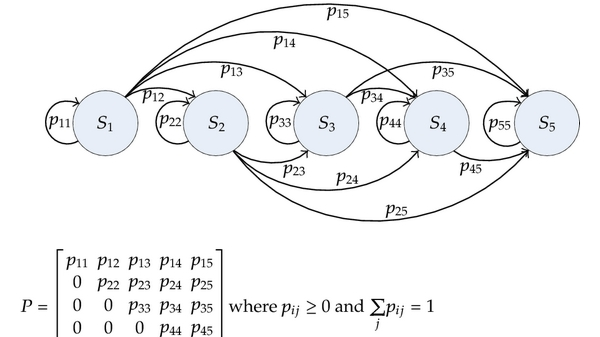
\includegraphics[width=14cm]{markov-chain-example}
	\caption{Example of a Markov Chain}
	\label{ex:markov-chain}
\end{figure}

Here, $P$ is the \textbf{Transition Matrix}. It contains all transition probabilities of the model. A \textbf{Markov Chain} (or Markov Process), is a tuple $(S, P)$, where $S$ is a set of states and $P$ is the transition matrix. A sequence $S_0, ..., S_n$ is called an \textbf{episode}.\\

From this Markov Chain, we can create a \textbf{Markov Reward Process}. This is defined as an extension of the tuple, with the elements $(S, P, R, \gamma)$. $S$ and $P$ mean the same thing as before. However, now we also have a reward function (recall that $R_s = \E[R_{t+1} | S_t=s]$) and a discount factor $\gamma \in [0, 1]$. How to then turn \ref{ex:markov-chain} into a MRP? Simply add reward values to each state in the Markov Chain. The rewards of each state can then be computed with the reward function.\\

Now let's introduce the \textbf{Bellman Equation} for MRP's. It is possible to rewrite the formula of the value function in the following way.

\begin{figure}[h]
	\begin{equation}
		\begin{aligned}
			v(s)&= \E[G_t | S_t = s]\\
				&= \E[R_{t+1} + \gamma (R_{t+2}, \gamma R_{t+3}, ...) | S_t = s]\\
				&= \E[R_{t+1} + \gamma G_{t+1} | S_t = s]\\
				&= \E[R_{t+1} + \gamma v(S_{t+1}) | S_t = s]\\
				&(= R_s + \gamma \sum_{s' \in S} P_{ss'}v(s'))
		\end{aligned}
	\end{equation}
	\caption{Bellman equation of the value function in a MRP}
	\label{form:bellman-value-mrp}
\end{figure}

Now it is possible to see that the value of a state is dependent on the immediate reward, and the return of neighboring states. This can then be computed using the transition matrix ($P_{ss'} > 0 \iff$ you can go from $s$ to $s'$). The bellman equation can then be written in matrix form, namely $v = R + \gamma Pv$.
This can be rewritten as $v = (I - \gamma P)^{-1} R$. This equation can be solved in $O(n^3)$, since a matrix inverse is necessary. For large MRP's, there are several iterative methods to solve this equation. For example,

\begin{itemize}
	\item Dynamic programming
	\item Monte-Carlo evaluation
	\item Temporal-Difference learning
\end{itemize}

These methods will be explained in later chapters.\\

\pagebreak

\section{Markov Decision Processes}

Finally, let's talk about the \textbf{Markov Decision Process}. This is an extension of the MRP, with properties $(S, A, P, R, \gamma)$. It introduces a new set, defining the actions that can be taken. The transition matrix $P^a$ and $R^a$ now also conditionally depend on the action.

\begin{figure}[h]
	\centering
	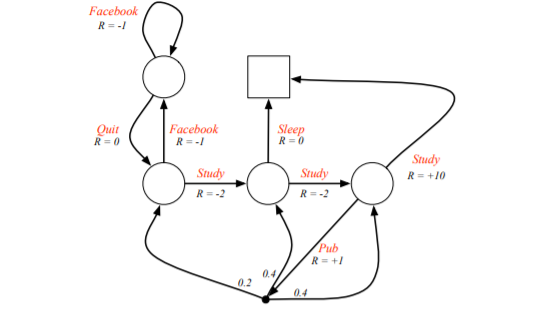
\includegraphics[width=15cm]{mdp-example}
	\caption{Example of a Markov Decision Process}
	\label{ex:mdp}
\end{figure}

\ref{ex:mdp} is an example of a Markov Decision Process. In the image you see that the rewards are now dependent on the actions, as previously explained. Now it is possible to talk about the behavior of an agent. In chapter 1, policies were mentioned. These determine the behavior of agents (like which action to take in which state).\\

Given an MDP and a policy $\pi$. The state sequence $S_0, S_1, ...$ is a Markov Process $(S, P^\pi)$ and the state and reward sequence $S_0, R_1, S_1, R_2, ...$ is a Markov Reward Process $(S, P^\pi, R^\pi, \gamma)$ where $P^\pi_{s, s'} = \sum_{a \in A} \pi(a | s)P^a_{s, s'}$ and $R^\pi_s = \sum_{a \in A} \pi(a | s)R^a_s$ (Law of Total Probability).\\

Similarly to the state-value function $v_\pi(s)$, let's now define the \textbf{action-value} function $q_\pi(s, a) = \E_\pi[G_t | S = s, A = a]$. This is the expected return starting from state s, taking action a, and then following policy $\pi$. In a RL problem, this is what we care about. The goal is to select the best action in a given state, in order to maximize the reward. If we have access to the $q$-values, it is the solution to the problem.\\

After deriving the Bellman equations for the MDP's, we end up with the following formulas.

\begin{figure}[h]
	\begin{equation}
		\begin{aligned}
			v(s)&= \E_\pi[G_t | S_t = s]\\
				&= \E_\pi[R_{t+1} + \gamma v(S_{t+1}) | S_t = s]\\
				&(= \sum_{a \in A}\pi(a|s)q_\pi(s, a))\\
				&(= \sum_{a \in A}\pi(a|s)\left(R^a_s + \gamma \sum_{s' \in S} P^a_{ss'}v_\pi(s')\right))
		\end{aligned}
	\end{equation}
	\caption{Bellman equation of the state value function in a MDP}
	\label{form:bellman-state-value-mdp}
\end{figure}

\begin{figure}[h]
	\begin{equation}
		\begin{aligned}
			q(s, a) &= \E_\pi[G_t | S_t = s, A_t = a]\\
					&= \E_\pi[R_{t+1} + \gamma q(S_{t+1}, A_{t+1}) | S_t = s, A_t = a]\\
					&(= R^a_s + \gamma \sum_{s' \in S} P^a_{ss'}v_\pi(s'))\\	
					&(= R^a_s + \gamma \sum_{s' \in S} P^a_{ss'}\sum_{a' \in A}\pi(a'|s')q_\pi(s', a'))	
		\end{aligned}
	\end{equation}
	\caption{Bellman equation of the action value function in a MDP}
	\label{form:bellman-action-value-mdp}
\end{figure}

The second-last form of formula \eqref{form:bellman-action-value-mdp} can be intuitively thought of as the following. Imagine we are taking a certain action in a state. Then, the environment might bring us into different successor states even if we take the action. So, we have to sum over all these possible successor states and use the law of total probability again to compute the action-values.\\

Now we can talk about optimality. The \textbf{optimal state-value} and \textbf{optimal action-value} functions are defined as $v_*(s) = \max_\pi v_\pi(s)$ and $q_*(s, a) = \max_\pi q_\pi(s, a)$. We can say $\pi \geq \pi'$ if $\forall s: v_\pi(s) \geq v_{\pi'}(s)$. The optimal value function specifies the best possible performance in the MDP. An MDP is "solved" when we know the optimal value. For any MDP, there always exist an optimal policy that is better or equal to all policies. This policy achieves both the optimal value function and the optimal action-value function.\\

An \textbf{optimal policy} can be found by maximizing over $q_*(s, a)$.

\begin{figure}[h]
	\begin{equation}
		\pi_*(a | s) =
		\begin{cases}
			1, & \text{if a = arg$\max_{a \in A} q_*(s, a)$}\\
			0, & \text{otherwise}
		\end{cases}
	\end{equation}
	\caption{Equation for an optimal policy}
	\label{form:optimal-policy}
\end{figure}

Thee optimal value functions are recursively related to the \textbf{Bellman Optimality Equations}. $v_*(s) = \max_a q_*(s, a)$ and $q_*(s, a) = R^a_s + \gamma \sum_{s' \in S} P^a_{ss'}v_*(s')$. Solving for these equations is difficult, since the Bellman Optimality Equation is non-linear. Generally, there is no closed form solution. However, there exist iterative methods to approximate the solution. Example of this are
\begin{itemize}
	\item Value Iteration
	\item Policy Iteration
	\item Q-learning
	\item Sarsa
\end{itemize}

\section{Advanced: Extensions to MDPs}

\subsection{Infinite and continuous MDPs}
\begin{itemize}
	\item Countably infinite state and/or action spaces
	\begin{itemize}
		\item Straightforward
	\end{itemize}
	\item Continuous state and/or action spaces
	\begin{itemize}
		\item Closed form for linear quadratic model (LQR)
	\end{itemize}
	\item Continuous time
	\begin{itemize}
		\item Requires partial differential equations
		\item Hamilton-Jacobi-Bellman (HJB) equation
		\item Limiting case of Bellman equation as time-step approaches 0
	\end{itemize}
\end{itemize}

\subsection{Partially observable MDPs}
A Partially Observable Markov Decision Process is an MDP with hidden states. It is a \textbf{hidden Markov model} with actions. A POMDP is a tuple $(S, A, O, P, R, Z, \gamma)$. We now also have $O$ representing a finite state of observations and $Z$ being an observation function $Z^a_{s'o} = \Prob[O_{t+1} = o | S_{t+1} = s', A_t = a]$.\\

Let's define a \textbf{history} $H_t$ being a sequence of actions, observations and rewards ($H_t = A_0, O_1, R_1, ..., A_{t-1}, O_t, R_t$). A \textbf{belief state} $b(h)$ is a probability distribution over states conditioned on the history h. $b(h) = (\Prob[S_t = s^1 | H_t = h], ..., \Prob[S_t = s^n | H_t = h])$.The history and belief state both satisfy the Markov property. A POMDP can be reduced to an (infinite) history tree and an (infinite) belief state tree.